\providecommand\lcode{\begingroup \small\urlstyle{tt}\Url}
\providecommand\lident{\begingroup \small\urlstyle{tt}\Url}
\providecommand{\NovilloSub}[1]{\raisebox{-.8ex}{$\scriptstyle#1$}}

\chapter{Propagating information using SSA\Author{D. Novillo}}
\numberofpages{6}
\chapterauthor{Novillo}

\graphicspath{{img/}{constant_propagation_is_easier/img/}{part3/constant_propagation_is_easier/img/}}

\section{Overview}

Several compiler transformations are based on the concept of
propagation.  Values or attributes generated at various producing
sites are propagated into other sites consumers of those values.
For instance, in constant propagation we are interested in
replacing loads from registers or memory into direct constant
references.

The most commonly used algorithm for constant propagation in SSA
form is known as SSA-CCP (Conditional Constant Propagation)
\cite{bib:wegman.ea-91}.  The basic idea is very simple,
constants are propagated by simulating the execution of the
program while keeping track of constant assignments.  Since the
program is in SSA form, every constant assignment of the form
$N_i = CST$ is recorded in an internal table indexed by SSA
index $i$.  During simulation, uses of $N_i$ are replaced with
$CST$, if that yields another constant value, the new constant
value is used for further propagation.  The simulation includes
keeping track of conditional predicates, if they are deemed to
have a statically computable value, the predicted branch is
simulated, and the others ignored.  Once simulation stops, the
values stored in the constant value table are replaced in the
program, expressions folded and the control flow graph adjusted
to account for predicted branches.

This chapter describes a generalization of this basic simulation
scheme used by SSA-CCP so that it can be used in other
transformations that can be expressed in terms of value
propagation.  The paper also describes some applications of this
\textit{propagation engine} to copy propagation and value range
propagation.  Section \ref{novillo:sec:prop-engine} describes the
propagation engine and its implementation in GCC.  Section
\ref{novillo:sec:copy-prop} describes an extension to the
traditional SSA based copy propagation that can also propagate
copies across conditionals.  Section \ref{novillo:sec:vrp}
describes an implementation of Value Range Propagation (VRP) in
GCC \cite{novillo:bib:patterson-95} and some infrastructure
changes for doing incremental updates to the SSA form.

\section{Propagation Engine}
\label{novillo:sec:prop-engine}

Propagation is performed by simulating the execution of every
statement that produces interesting values.  In this context, an
\textit{interesting} value is anything that the specific
implementation is looking to propagate: constants in SSA-CCP,
copies in copy propagation, range information in VRP, etc.

Both control and data flow are simulated using two separate work
lists: a list of control flow edges (\textit{CFG work list}) and a
list of def-use edges (\textit{SSA work list}).  Simulation proceeds as
follows:

\begin{enumerate}
\item	Initially, every edge in the CFG is marked not executable
	and the CFG work list is seeded with all the statements in
	the first executable basic block.  The SSA work list is
	initially empty.

\item	\label{novillo:prop-return-value}A basic block $B$ is
	taken from the CFG work list and every statement $S$ in
	$B$ is evaluated with a call to a user-provided callback
	function (\lident{ssa_prop_visit_stmt}).  This evaluation
	may produce 3 results:

	\lident{SSA_PROP_INTERESTING}: $S$ produces a
	value deemed interesting by the callback function and
	that can be computed at compile time.  When this occurs,
	\lident{ssa_prop_visit_stmt} is responsible for
	storing the value in a separate table and returning a
	single SSA name $N_i$ associated to that
	value\footnote{In some propagation problems it may be
	useful to allow statements to return more than one
	interesting name.}.

	All the statements with immediate uses of $N_i$ are then
	added to the SSA work list so that they can also be
	simulated.  Furthermore, if $S$ is a conditional jump and
	\lident{ssa_prop_visit_stmt} has determined that it
	always takes the same edge $E$, then only the basic block
	reachable through $E$ is added to the CFG work list.

	If $S$ is not a conditional jump, or if $S$ is a
	conditional jump whose value cannot be determined, all
	the immediate successors of $B$ are added to the CFG
	work list.

	\lident{SSA_PROP_NOT_INTERESTING}: Statement $S$
	produces nothing of interest and does not affect any of
	the work lists.  The statement may be simulated again if
	any of its input operands change in future iterations of
	the simulator.

	\lident{SSA_PROP_VARYING}: The value produced
	by $S$ cannot be determined at compile time and further
	simulation of $S$ is not needed.  If $S$ is a conditional
	jump, all the immediate successors of $B$ are added to
	the CFG work list.  Once a statement yields a varying
	value, it is never simulated again.

	Once all the statements in basic block $B$ have been
	simulated, its statements are not traversed again.
	Statements are only visited more than once if they are
	added to the SSA work list when visiting other statements.

\item	If block $B$ has any $\phi$ nodes, they are simulated
	with a call to the callback function
	\lident{ssa_prop_visit_phi}.  As opposed to regular
	statements, $\phi$ nodes are \textit{always} simulated
	every time $B$ is added to the CFG work list.  This is
	because $\phi$ nodes receive their inputs from different
	incoming edges, so every time a new edge is marked
	executable, a new argument of each $\phi$ node will
	become available for simulation.

	It is up to \lident{ssa_prop_visit_phi} to only
	consider $\phi$ arguments flowing through executable
	edges (marked with flag \lident{EDGE_EXECUTABLE}). The
	return value from \lident{ssa_prop_visit_phi} has the
	same semantics described in \ref{novillo:prop-return-value}.

	Also, the evaluation of $\phi$ nodes is different from
	other statements.  A $\phi$ node is a merging point
	of potentially different values from different SSA
	names.  In general, the resulting value of a $\phi$ node
	will be the ``intersection'' of all the incoming values.
	Each propagator will have a different concept of
	intersection according to its own lattice value rules.

\item	Simulation terminates when both work lists are drained.
\end{enumerate}

For efficiency of implementation, the SSA work list is split in
two separate lists: one to hold all the SSA names with a result
of \lident{SSA_PROP_VARYING} and another one to hold those with
\lident{SSA_PROP_INTERESTING} values.  The rationale is that
the majority of names will not actually yield interesting values,
so it is more efficient to dispose of the varying values by
simulating the affected statements as soon as possible.

\subsection{Keeping track of propagated values}

As discussed earlier, during propagation two user provided
functions are called: \lident{ssa_prop_visit_stmt} and
\lident{ssa_prop_visit_phi}.  The propagator itself is only
interested in the three return values to determine which blocks
and statements to add in the work lists.  However, the real work
is in keeping track of propagated values.  Every interesting
value produced by simulation must be associated to a single SSA
name $N_i$, but the final values must not be replaced in the IL
until propagation has finished.  During propagation, names may
get more than a single value.

Once propagation has finished, final values for every SSA name in
the program are available in the array $PV$, which holds propagated
values indexed by SSA index.  If name $N_i$ has final value $V$
then $PV[i] == V$.


To summarize, every propagation algorithm should define three
basic elements:

\begin{enumerate}
\item	An array of values $V$ of type \lident{prop_value_t}
	indexed by SSA index number.

\item	Statement simulation (\lident{ssa_prop_visit_stmt}).
	Evaluates the expression computed by the statement, if
	the statement produces an interesting result, it must be
	in the form of an SSA name $N_i$.  The produced value is
	stored in $V[i]$ and $N_i$ is returned to the propagator
	engine so that its def-use edges can be added to the SSA
	work list.

	If the statement is a conditional jump and it is possible
	to compute which edge $E$ will be taken, $E$ is returned
	so that its destination basic block can be added to the
	CFG work list.  Otherwise, all outgoing edges are added
	to the list.

\item	$\phi$ node simulation (\lident{ssa_prop_visit_phi}).
	Similar to \lident{ssa_prop_visit_stmt} but the
	evaluation is a user-defined merge operation of all the
	values coming in through executable edges.
\end{enumerate}

Once an implementation for \lident{ssa_prop_visit_stmt} and
\lident{ssa_prop_visit_phi} exists, propagation is done with a
call to \lident{ssa_propagate}.

%---------------------------------------------------------------------------

\section{Copy Propagation}
\label{novillo:sec:copy-prop}

Copy propagation in SSA form is, in principle, very simple.  Given
the assignment $x_5 = y_4$, all we need to do is traverse all the
immediate uses of $x_5$ and replace them with $y_4$.  However,
such approach will not be able to propagate copies past $\phi$
nodes, particularly those involved in loops.  Note that it may be
debatable whether aggressive copy-propagation is desirable, as
this may have negative effects on passes like register allocation
(due to increased register pressure), but the current
implementation sticks to the simplistic metric of maximizing the
number of propagated copies.

\subsection{Lattice for copy propagation}

Copy propagation can be described as the problem of propagating
the \textit{copy-of} value of SSA names.  Given

\begin{center}
\parbox{1in}{\lgrindfile{copy-prop-1.c.tex}}
\end{center}

We say that y$_4$ is a \textit{copy-of} z$_6$ and x$_5$ is a
\textit{copy-of} $y_4$.  The problem with this representation is
that there is no apparent link from x$_5$ to z$_6$.  So, when
visiting assignments in \lident{copy_prop_visit_stmt}, we assign
copy-of values instead of the direct copy.  If a variable is not
found to be a copy of anything else, its copy-of value is itself.
So, in this case we would have y$_4$ copy-of z$_6$ and x$_5$
copy-of z$_6$.  At the end of propagation, uses of x$_5$ and y$_4$
will be replaced with z$_6$.


Propagation must also be able to propagate copies exposed by
$\phi$ nodes.  For instance,

\begin{center}
\parbox{2in}{\lgrindfile{copy-prop-2.c.tex}}
\end{center}

Should result in z$_9$ being a copy of z$_6$.  The implementation
of \lident{ssa_prop_visit_phi} only needs to check the copy-of
values of every executable $\phi$-argument.  If they all match,
then the LHS of the $\phi$ node (z$_9$ in this case) can have its
copy-of value set to the common copy-of value.  Otherwise, the
value of the $\phi$ node is considered varying and the copy-of
value of the name on the LHS is itself.  So, when visiting the
$\phi$ node for z$_9$, the propagator finds x$_5$ copy-of z$_6$
and y$_4$ copy-of z$_6$, which means that z$_9$ is copy-of z$_6$.

The following example shows a more complex situation where copy
relations may be obfuscated by loops.  Note that the actual visit
ordering depends on the shape of the CFG and immediate uses, the
ordering used here is meant for illustration only:

\begin{center}
\parbox{2in}{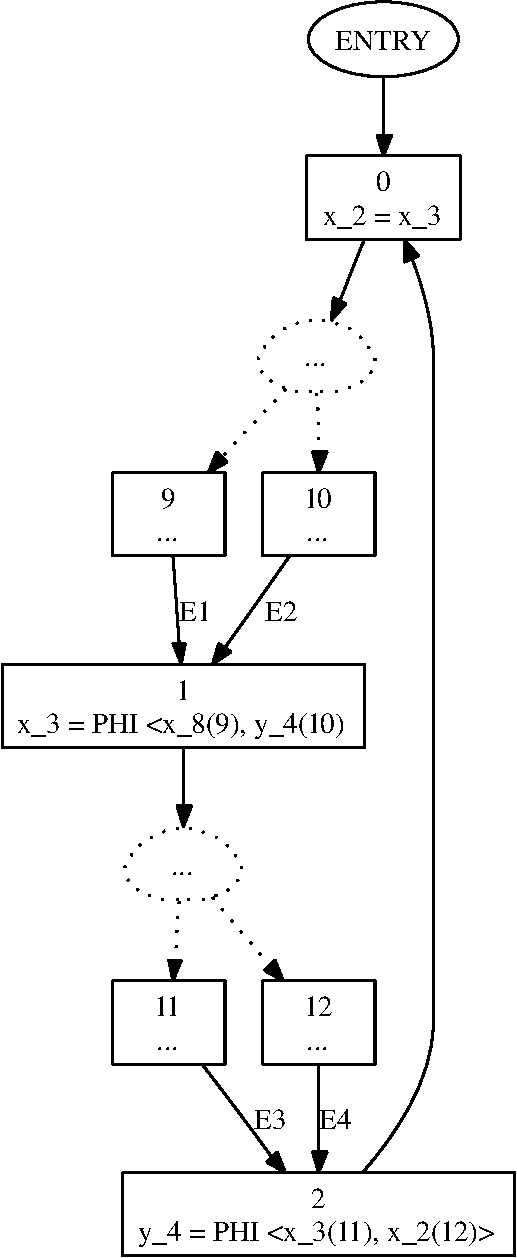
\includegraphics[height=4in]{copy-prop-3}}
\end{center}

\begin{enumerate}
\item	The first time we visit block $1$, edge E1 is marked
	executable, but edge E2 is not.  Therefore, the visit to
	x$_3$ = $\phi$<x$_8$(9), y$_4$(10)> results in x$_4$
	copy-of x$_8$.  Since x$_3$ has changed to a new value,
	the SSA edges for x$_3$ are added to the work list ($1
	\rightarrow 2$ and $1 \rightarrow 0$).

\item	Visit SSA edge $1 \rightarrow 2$: y$_4$ = $\phi$
	<x$_3$(11), x$_2$(12)>.  Assume that edge E3 is marked
	executable, and edge E4 is marked not executable.  This
	yields y$_4$ copy-of x$_8$, because x$_3$ is copy-of
	x$_8$.  The SSA edge $2 \rightarrow 1$ for y$_4$ is added
	to the work list.

\item	Visit SSA edge $1 \rightarrow 0$: x$_2$ = x$_3$.  This
	yields x$_2$ copy-of x$_8$.  The SSA edge $0 \rightarrow
	2$ for x$_2$ is added to the work list.

\item	Visit SSA edge $2 \rightarrow 1$: x$_3$ =
	$\phi$<x$_8$(9), y$_4$(10)>.  This time both edges E1 and
	E2 are marked executable.  Since x$_3$ has not changed
	its copy-of value, no edges are added to the work list.

\item	Visit SSA edge $1 \rightarrow 0$: x$_2$ = x$_3$.  The
	value of x$_2$ changes to copy-of x$_8$.  Therefore, SSA
	edge $0 \rightarrow 2$ for x$_2$ is added to the work
	list.

\item	Visit SSA edge $0 \rightarrow 2$.  This time both edges
	E3 and E4 are marked executable.  Since both arguments
	are copy-of x$_8$, the value of y$_4$ doesn't change.

\item	Work lists are drained.  Iteration stops.
\end{enumerate}

The straightforward implementation of copy propagation, would
have needed multiple passes to discover that x$_3 \rightarrow$
x$_8$.  But the iterative nature of the propagation engine
prevents that.  Moreover, this kind of propagation will only
iterate over the subset of statements affected, not the whole
CFG.

\section{Value Range Propagation (VRP)}
\label{novillo:sec:vrp}

This transformation is similar to constant propagation but
instead of propagating single constant values, it propagates
known value ranges.  For instance, the code in Figure
\ref{novillo:fig:vrp-1} is extracted from a typical expansion of
bound checking code in languages like Java. Notice how the bound
checking done at line 3 is not really necessary as variable $i$
is guaranteed to take values in the range [$0$, a->len].

\begin{figure}
    \centering
    \parbox{2in}{\lgrindfile{vrp-1.c.tex}}
    \caption{Bound checking code generated by the compiler.}
    \label{novillo:fig:vrp-1}
\end{figure}

Value range propagation works in two main phases:

\begin{enumerate}
\item	Range Assertions.  Some expressions like predicates in
	conditional jumps, pointer dereferences or taking the
	absolute value of a variable imply something about the
	range of values that their result may take.  For
	instance, the expression \lcode{if (a_5 > 10) ...}
	implies that every use of a$_5$ inside the if will be
	guaranteed to use values in the range [$11$, +INF].

	For every expression in this category, the compiler
	generates a new expression code (\lcode{ASSERT_EXPR})
	that describes the guaranteed range of values taken by
	the associated name.

\item	Range Propagation.  Once \lcode{ASSERT_EXPR} instructions
	have been inserted, the SSA propagation engine is used to
	evaluate the program.  After propagation, every SSA name
	created by the program will have a range of values
	associated with it.  Those ranges are then used to
	eliminate conditional jumps made superfluous by the new
	range information.
\end{enumerate}

\subsection{Inserting range assertions}

Certain expressions found in the code give us information about
the range of values that may be taken by the operands involved in
the expression.  For instance, consider the code fragment in
Figure \ref{novillo:fig:assert-expr-before}.

\begin{figure*}
    \centering
    \subfigure[Before inserting assertions.]{
	\label{novillo:fig:assert-expr-before}
	\parbox{2in}{\lgrindfile{vrp-2.c.tex}}
    }
    \ \hspace{3em}
    \subfigure[After inserting assertions.]{
	\label{novillo:fig:assert-expr-after}
	\parbox{2.5in}{\lgrindfile{vrp-3.c.tex}}
    }
    \caption{Preparing the program for Value Range Propagation.}
\end{figure*}

Since pointer p$_4$ is dereferenced at line $6$, we know that the
NULL test at line $8$ must always fail.  Similarly, the use of
a$_5$ at line $12$ is guaranteed to always use the constant value
$10$.  However, we cannot guarantee that \textbf{all} uses of
p$_4$ and a$_5$ will always have a known value.  For instance,
we have no way of knowing at compile time whether the NULL test
for p$_4$ at line $3$ will succeed or not.  Similarly, the use of
a$_5$ at line $14$ does not use a known value.

The technique used by VRP to overcome this problem is to create
new SSA names to which we can pin the range information that we
want to propagate.  The compiler generates a new expression called
\lcode{ASSERT_EXPR} that captures this information and stores it
into a new SSA name.  When the compiler finds an expression that
contains interesting range information for name $N_i$, it
builds a predicate P describing that range and generates
the assignment \lcode{N_j = ASSERT_EXPR <N_i, P>}.  This
expression means that variable $N_j$ has the same value as $N_i$
\textbf{and} that value is guaranteed to make predicate P
evaluate to \textit{true}.

Therefore, for the code in Figure
\ref{novillo:fig:assert-expr-before}, the compiler inserts the
assertions found in Figure \ref{novillo:fig:assert-expr-after}.
The pointer dereference in line $6$ produces the assertion
p$_5$ = \lcode{ASSERT_EXPR <}p$_4$, p$_4$ != $0$\lcode{>}.  With
this conversion, all uses of p$_5$ are guaranteed to be uses of a
non-NULL pointer.  Similarly, uses of a$_6$ are guaranteed to use
the constant value $10$.

\subsection{Incremental updates of the SSA form}

Since range assertion expressions are inserted once the program
is in SSA form, it must be updated before ranges are propagated.
Each expression $N_i$ = \lcode{ASSERT_EXPR <}$N_j$, P\lcode{>}
creates a mapping from the existing name $N_j$ to the new name
$N_i$.

As assertions are inserted in the IL, a replacement mapping is
built.  In the example code of Figure
\ref{novillo:fig:assert-expr-after}, the compiler will build two
mappings, namely p$_5 \rightarrow$ p$_4$ and a$_6 \rightarrow$
a$_5$.  Once all the assertions have been inserted, the SSA form 
can be incrementally updated by applying all the name mappings.

The mechanics of the updating process are a little more
elaborate than this, but in essence all it does is search and
replace inside the sub-regions of the CFG affected by the
existing names and their replacements.

\subsection{Propagating ranges}

\begin{figure}
    \centering
    \parbox{2in}{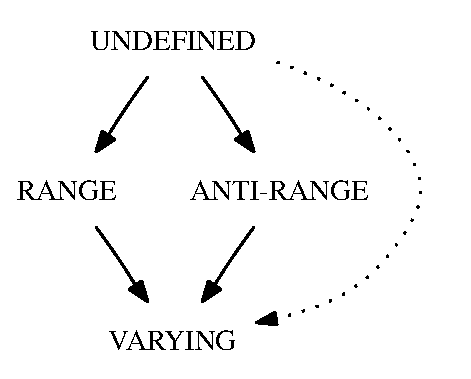
\includegraphics[height=2in]{vrp-4}}
    \caption{Lattice values used for range propagation.}
    \label{novillo:fig:vrp-lattice}
\end{figure}

The range propagation lattice has 4 values as shown in Figure
\ref{novillo:fig:vrp-lattice}.  As is the case with other
propagation problems, the only valid transitions are those that
move downward in the lattice.  If we were to allow transitions in
different directions, we would risk infinite loops during
propagation.

Lattice values \textsc{RANGE} and \textsc{ANTI-RANGE} are exactly
the same in terms of propagation, they both represent known
range values for the associated SSA names.  The key difference is
in the semantics of the actual value when evaluating expressions.

Two types of statements are considered interesting by the
propagator:

\begin{enumerate}
\item	Assignments of the form $N_i$ = EXPR, where EXPR is of
	an integral or pointer type.  The expression is evaluated
	and if it results in a useful range, its value is
	associated to $N_i$.
	
	Naturally, the more common sources of useful range
	information are \lcode{ASSERT_EXPR}s, but other
	expressions may also provide useful ranges.  For
	instance, if EXPR is $42$, then we can set the range of
	$N_i$ to $[42, 42]$.  Similarly, expressions involving
	names with known ranges may yield useful information.

\item	Conditional branches are also evaluated.  If the
	controlling predicate includes names with known ranges,
	only the taken edges are added to the CFG work list.
\end{enumerate}

Evaluation of $\phi$ nodes uses the usual shortcut of ignoring
arguments coming through non-executable edges.  Given two
arguments with ranges VR0 and VR1:

\begin{enumerate}
\item	If VR0 and VR1 have an empty intersection the resulting
	range is set to VARYING.

\item	Otherwise, the resulting range is VR0 $\bigcup$ VR1.
\end{enumerate}

Propagation continues while names change from one state to the
other.  Once all the basic blocks have been simulated and no
state transitions occur, simulation stops.
